\section{VM Volume storage}

\begin{frame}[t]{Intro}

	\note[item]{Σε μεγάλες εγκαταστάσεις, ξεφεύγουμε από το κλασσικό 
		μοντέλο του PC μας (το μηχάνημα έχει το σκληρό του δίσκο).  
		Συγκεκριμένα σε μια cloud υποδομή έχουμε:}
	\note[item]{\click}
	\note[item]{To VM που τρέχει σε φυσικούς κόμβους}
	\note[item]{\click}
	\note[item]{τον εικονικό σκληρό του δίσκo, το κλασσικό /dev/sda/}
	\note[item]{\click}
	\note[item]{Και τους storage servers}
	\note[item]{\click}
	\note[item]{Το ερώτημα είναι λοιπόν, πως το VM θα αποθηκεύει τα δεδομένα 
		του; Παράλληλα, τι γίνεται στην περίπτωση που θέλουμε *και* τα εξής;}
	\note[item]{\click}
	\note[item]{Εξήγησε τους όρους}

	\pause
	\includegraphics[width=.2\textwidth]{images/vm.jpg}\pause {\Huge +} 
	\includegraphics[width=.1\textwidth]{images/hdd.jpg}
	\pause
		 \includegraphics[width=.05\textwidth]{images/link.png}
		 \includegraphics[width=.15\textwidth]{images/cloud-server1.jpg}

	\pause\dspc
	\begin{itemize}
		\item Policy enforcement?
		\item Storage agnosticity?
	\end{itemize}

	\note[item]{Δηλαδή εφαρμογή δικών μας πολιτικών, χρήση οποιουδήποτε τύπου 
		storage}
\end{frame}

\begin{frame}{Our solution}

	{\Large Archipelago (many nodes)}

	\centering\makebox[\textwidth]{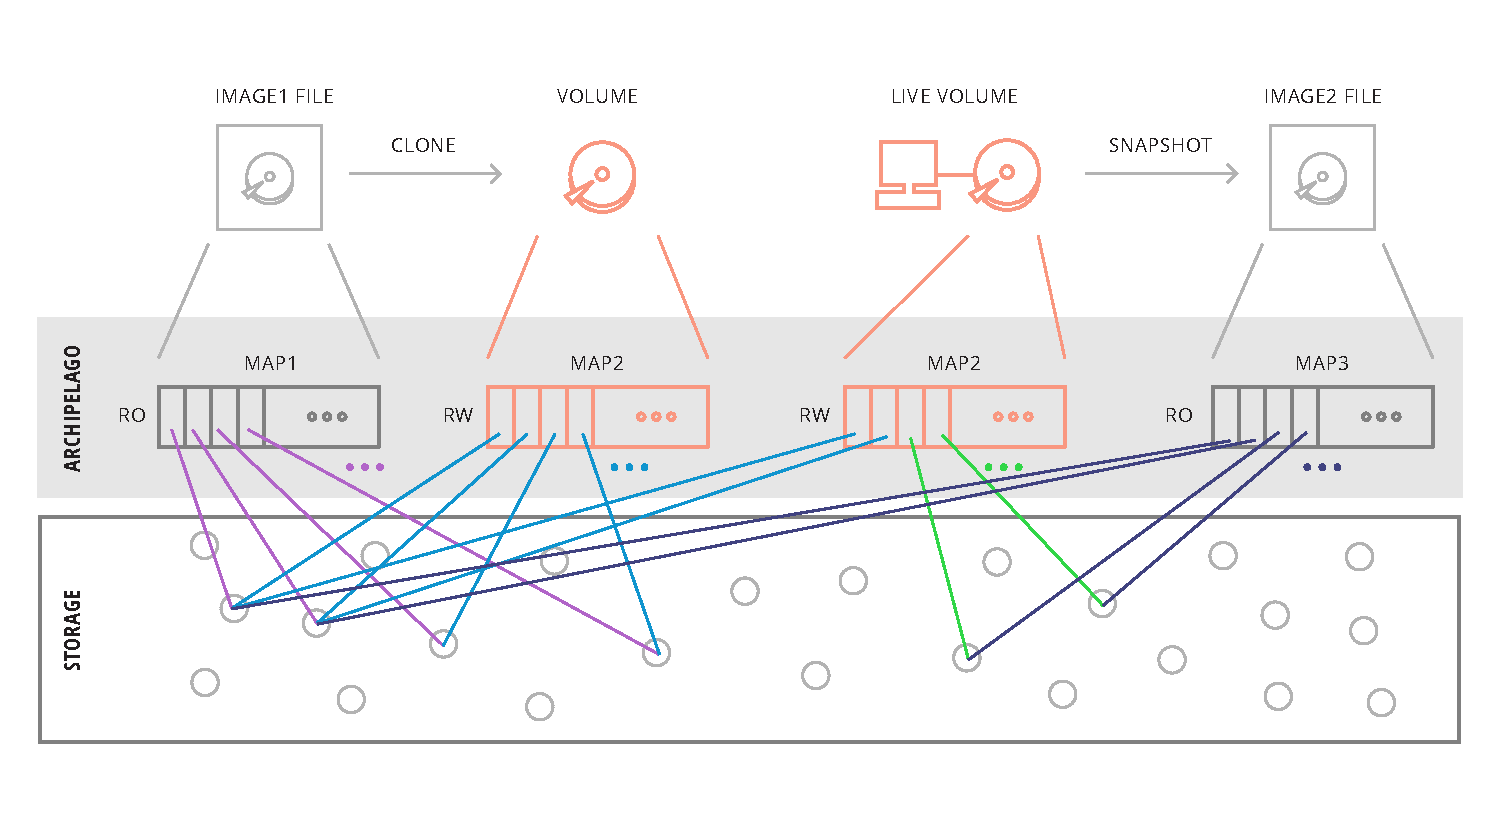
\includegraphics[width=0.8\textwidth]{images/archipelago-composition.pdf}}

	\spc

	Key features:
		1) Software-defined
		2) Distributed
		3) Modular
		4) Copy-On-Write
		5) Storage agnostic

	\note{Η λύση που χρησιμοποιήσαμε είναι το Archipelago}
	\note[item]{Πιο συγκεκριμένα, το Αρχιπέλαγο τρέχει στον host κόμβο. Είναι 
		ΑΚRIBΩΣ κάτω από τον σκληρό δίσκο του VM, το /dev/vda1. Τα δεδομένα 
		είναι στο storage}
	\note[item]{
		\begin{itemize}
			\item Software-defined: με το software ΟΡΙΖΕΙΣ το storage (εφαρμογή 
				policy, χρήση διαφορετικού storage για κάθε volume)
			\item τρέχει σε πολλούς κόμβους
			\item αποτελείται από διακριτά κομμάτια
			\item χρησιμοποιεί Copy-on-Write policy. NA αναφέρουμε εδώ ότι το 
				copy on write είναι μια πολιτική αντιγραφής ενός αντικειμένου.  
				To αντικείμενο σπάει σε κομμάτια τα οποία αντιγράφονται ΜΟΝΟ 
				όταν πάει να γράψει σε κάποιο από αυτά.
			\item μπορούμε χρησιμοποιήσουμε ότι storage θέλουμε
		\end{itemize}
	}
\end{frame}

\begin{frame}{Archipelago Architecture (single node)}
	\begin{center}
		  \makebox[\textwidth]{\includegraphics[width=0.9\paperwidth]{images/new_sxima_numbered.pdf}}
	\end{center}

	\note[item]{Βλέπουμε τώρα το Αρχιπέλαγο σε ένα κόμβο. Όλα είναι userspace 
		διεργασίες, μόνο ο xsegbd είναι kernel driver (όλα είναι PEERS)}
	\note[item]{Ας δουμε τη διαδρομή ενός IO request. To VM στέλνει αίτημα στο 
		δίσκο του. Ποιον δίσκο; /dev/vda1}
	\note[item]{ο δίσκος είναι εικονικός, θα το δει ο hypervisor (ο υπεύθυνος 
		για το virtualization του Virtual Machine) και θα το στείλει στον δίσκο 
		που το έχουμε πει.  (xsegbd)}
	\note[item]{Ο xsegbd είναι kernel driver και θα στέλνει τo αίτημα στο 
		userspace κομμάτι του Αρχιπελάγους το οποίο αποφαίνεται για τα 
		αντικείμενα τα οποία αντιστοιχούν στο αίτημα. Στο αίτημα αυτό θα 
		αναφέρεται ότι προέρχεται από το volume foo.}
	\note[item]{το παίρνει ο vlmc, ρωτάει τον mapper, από ποια αντικείμενα 
		αποτελείται; λέει ότι είναι το foo}
	\note[item]{μετά τα ζητάει από το storage μέσω των blockers. ΤΩΡΑ ΜΙΛΑΜΕ 
		για την έλλειψη στα δεξια}
\end{frame}

\begin{frame}{RADOS}

	The object store component of a promising technology
	\dspc
	Key features:
	\begin{itemize}
		\item Replication
		\item Fault tolerance
		\item Self-management
		\item Scalability
		\item Uses commodity hardware
	\end{itemize}

	\note{Αν και είμαστε storage agnostic, χρησιμοποιούμε ένα σημαντικό storage 
		backend, το RADOS. To rados είναι το object store component μιας πολλά 
		υποσχόμενης τεχνολογίας που μας δίνει τα εξής:
		\begin{itemize}
			\item Αντίγραφα ασφαλείας των δεδομένων
			\item Ανοχή στο χάσιμο αποθηκευτικών κόμβων
			\item Load balancing και αυτοδιαχείριση
			\item ειναι κλιμακώσιμο
			\item χρησιμοποιεί απλό hardware
		\end{itemize}
	}
	\note[itemize]{υ.γ. αντικείμενα είναι ονοματοδοτούμενη ποσότητα 
		πληροφορίας}
\end{frame}

\begin{frame}{Thesis motivation}
	\begin{itemize}
		\item RADOS has speed issues: Bandwidth < 7MB/s, Latency \mytilde10ms
		\item Request type: Block size: 4KB, parallel requests: 16
		\item Qualitative benchmark that depicts a hard workload
	\end{itemize}
	\spc
	Thesis goal: Mitigate RADOS speed issues.
	\dspc
	Observation:\\
	VM with page-cache of host enabled: Bandwidth > 90MB/s, Latency < 1ms
	\dspc
	Page-cache is great but it has many limitations:
	\begin{itemize}
		\item KVM and Linux kernel dependent (we REALLY want to avoid this)
		\item Unaware of CoW policies
		\item Difficult to manage
	\end{itemize}

	\note[item]{Αυτό το περίπλοκο σύστημα όμως δεν είναι αρκετά ταχύ.  Από 
		πραγματικές μετρήσεις σε ένα VM έχουμε ότι:...}
	\note[item]{Αυτά τα αποτελέσματα δεν είναι καλά}
	\note[item]{Στόχος διπλωματικής, απάλειψη του αντίκτυπου της επίδοσης του 
		RADOS στο Αρχιπέλαγο}
	\note[item]{Παρατηρήσαμε ότι αν ενεργοποιήσουμε την page cache έχουμε...}
	\note[item]{Η page-cache όμως έχει σοβαρούς περιορισμούς}
	\note[item]{Επίση, εμείς μπορεί να θέλουμε να cach-άρουμε σε ssd, να 
		κάνουμε replication, να έχουμε επιλεγόμενα επίπεδα αξιοπιστίας για κάθε 
		VM}
\end{frame}

